\section{The Receiver}\label{sec:receiver}

\begin{figure}[!htbp]\centering
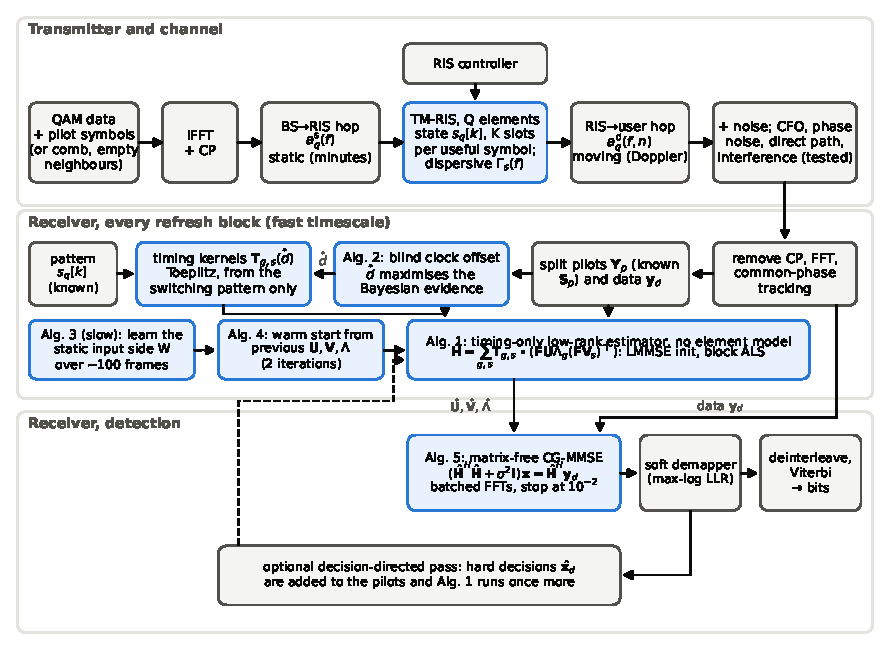
\includegraphics[width=0.95\textwidth]{figP_pipeline.pdf}
\caption{Complete system and receiver pipeline. Shaded blocks are the proposed receiver
components; each is an algorithm of Section~\ref{sec:receiver}. The receiver uses the
switching pattern (A1) and never the element model.}
\label{fig:pipeline}
\end{figure}

\subsection{Architecture}
Fig.~\ref{fig:pipeline} shows the complete pipeline. The transmitter sends $N_p$ pilot
OFDM symbols followed by data, either as full pilot symbols or as comb pilots with empty
neighbouring resource elements (Section~\ref{sec:res-pilot} shows the two are
equivalent and that data next to pilots is not). The receiver removes the cyclic prefix,
applies the FFT and, under mobility, corrects one common phase per symbol (A7). It then
(i) builds the timing kernels $\bm T_{g,s}$ from the known pattern; (ii) estimates the RIS
clock offset $\hat d$ blindly from the pilots (Algorithm~\ref{alg:offset}) and shifts the
kernels; (iii) estimates the coupling matrix in factored form (Algorithm~\ref{alg:est}),
either from scratch or warm-started from the previous refresh block (Algorithm~\ref{alg:warm}),
optionally with the static input side learned on a slow timescale (Algorithm~\ref{alg:learn});
(iv) equalizes the data matrix-free by conjugate gradients (Algorithm~\ref{alg:cg}); and
(v) computes max-log LLRs from its own estimate for a soft-input channel decoder. One
optional decision-directed (DD) pass reuses hard decisions as additional pilots. All
blocks use the factored model~\eqref{eq:model}; the $M\times M$ matrix is never formed.

\subsection{Timing-only low-rank estimation}\label{sec:est}
\emph{Model and prior.} Each hop's response is delay-limited to $[0,\tau_{\max}]$. We
represent it with the first $L$ discrete prolate spheroidal sequences (DPSS) of the
bandwidth--delay product $M\Delta f\tau_{\max}$~\cite{slepian1978,zemen2005}: $\bm F\in\mathbb C^{M\times L}$
holds the leading eigenvectors of $R_{nm}=e^{-j\pi(n-m)\Delta f\tau_{\max}}\mathrm{sinc}((n-m)\Delta f\tau_{\max})$,
and $\bm\lambda\in\mathbb R^{L}$ their eigenvalues normalized to unit sum. The DPSS basis is
the best $L$-dimensional subspace for responses with delays uniform in $[0,\tau_{\max}]$ and
has no delay grid to fall off. The eigenvalues serve as prior variances: coefficient $l$
of any hop response has prior variance $\varsigma\lambda_l$, with the scale $\varsigma$ set by
moment matching on the pilots. This prior is what keeps the estimator stable when $L$ is
larger than the effective number of delay dimensions ($M\Delta f\tau_{\max}+1\approx3.3$ at
$M=256$, $\tau_{\max}=0.3\,\mu$s, while $L=16$).

\emph{Observation model.} Pilot symbol $p$ is $\bm s_p\in\mathbb C^M$ with received $\bm y_p$.
By Corollary~\ref{cor:fft}, $\bm H\bm s_p$ is linear in each of $\bm U$, $\bm V_s$ and $\bm\Lambda_g$
when the others are fixed, with regressors built from
$\bm G_{g,s,p}=\bm T_{g,s}(\bm s_p\odot\bm F)\in\mathbb C^{M\times L}$, computed once by FFT:
\begin{align}
\bm H\bm s_p&=\textstyle\sum_g\sum_{a=1}^{r}(\bm F\bm u_a)\odot\big[\textstyle\sum_s\bm G_{g,s,p}\bm V_s\bm\Lambda_g^{\top}\big]_{:,a}\label{eq:linU}\\
&=\textstyle\sum_g\sum_s\sum_{b=1}^{r}\big[(\bm F\bm U\bm\Lambda_g)_{:,b}\odot\bm G_{g,s,p}\big]\bm v_{s,b}\label{eq:linV}\\
&=\textstyle\sum_g\sum_{a,b}\big[(\bm F\bm u_a)\odot(\textstyle\sum_s\bm G_{g,s,p}\bm V_s)_{:,b}\big]\,[\bm\Lambda_g]_{ab},\label{eq:linL}
\end{align}
which are linear in $\bm U$, in $\bm V_s$ and in $\bm\Lambda_g$, respectively.
Stacking the $N_p$ pilots gives, for each block $\bm\theta\in\{\vect\bm U,\vect[\bm V_1;\bm V_2],\vect\{\bm\Lambda_g\}\}$,
a linear model $\bm y=\bm A_{\bm\theta}\bm\theta+\bm w$, $\bm y=\vect[\bm y_1,\dots,\bm y_{N_p}]$.
With prior $\bm\theta\sim\mathcal{CN}(\bm 0,\bm P)$, $\bm P=\diag(\bm p)$, the LMMSE update is computed in
the numerically stable form
\begin{equation}
\hat{\bm\theta}=\bm P^{1/2}\big(\bm P^{1/2}\bm A_{\bm\theta}^{\mathsf H}\bm A_{\bm\theta}\bm P^{1/2}+\sigma^2\bm I\big)^{-1}\bm P^{1/2}\bm A_{\bm\theta}^{\mathsf H}\bm y,
\label{eq:lmmse}
\end{equation}
which remains well posed when some prior variances are tiny. The $\bm\Lambda$ step is a
convex least-squares problem with a small ridge ($10^{-3}$ of the mean diagonal of
$\bm A^{\mathsf H}\bm A$).

\emph{Initialization.} Ignoring the low-rank coupling between groups, $\bm H\approx\sum_s(\sum_g\bm T_{g,s})\circ(\bm F\bm C_s\bm F^{\top})$
is linear in the two $L\times L$ delay matrices $\bm C_s$. Its LMMSE estimate with prior
$\varsigma(\bm\lambda\otimes\bm\lambda)$ is exact for identical patterns ($G=1$), and its SVD,
$[\hat{\bm C}_1\;\hat{\bm C}_2]=\bm Y\bm\Sigma\bm W^{\mathsf H}$, initializes
$\bm U=\bm Y_{:,1:r}\bm\Sigma_r^{1/2}$ and $[\bm V_1;\bm V_2]=\bm W^{*}_{:,1:r}\bm\Sigma_r^{1/2}$, $\bm\Lambda_g=\bm I$.
An earlier version kept the pooled linear estimate as a fallback whenever it fitted the pilots
better. The ablation (Section~\ref{sec:res-ablation}) showed that this rule is itself an overfitting trap: the linear
model has more freedom, fits the pilots better and predicts worse, and on TDL channels at 30\,dB it was chosen in
30--57\% of channels and increased the gap. On fresh channels (pre-registered), removing it never made the gap worse
and reduced it by up to $0.25\pm0.17$\,bit/s/Hz; Algorithm~\ref{alg:est} therefore always returns the low-rank
estimate. The alternating iterations converge within one or two iterations from the SVD initialization, while random
initializations are 3--5 times worse, so the initialization matters more than the iteration count.

\begin{algorithm}[!htbp]
\caption{Timing-only low-rank estimation}\label{alg:est}
\begin{algorithmic}[1]
\Require pilots $\bm Y,\bm S$; kernels $\{\bm T_{g,s}\}$; DPSS $\bm F,\bm\lambda$; $\sigma^2$; rank $r$; iterations $I$ (20)
\State $\bm G_{g,s,p}\gets\bm T_{g,s}(\bm s_p\odot\bm F)$ by FFT \Comment{once}
\State $[\hat{\bm C}_1,\hat{\bm C}_2]\gets$ LMMSE of the pooled linear model, prior $\varsigma(\bm\lambda\otimes\bm\lambda)$
\State $\bm U,\bm V_1,\bm V_2\gets$ rank-$r$ SVD of $[\hat{\bm C}_1\;\hat{\bm C}_2]$; $\bm\Lambda_g\gets\bm I$; prior of $\bm U,\bm V_s$ columns $\propto\bm\lambda$
\For{$i=1,\dots,I$}
  \State $\{\bm\Lambda_g\}\gets$ ridge least squares (convex) \Comment{(linear in $\bm\Lambda$)}
  \State $\bm U\gets$ LMMSE~\eqref{eq:lmmse} \Comment{$Lr$ unknowns}
  \State $[\bm V_1;\bm V_2]\gets$ LMMSE~\eqref{eq:lmmse} \Comment{$2Lr$ unknowns}
\EndFor
\State $\hat{\bm H}\gets\sum_{g,s}\bm T_{g,s}\circ((\bm F\bm U)\bm\Lambda_g(\bm F\bm V_s)^{\top})$ (kept factored)
\State \Return $\hat{\bm H}$ \Comment{no pilot-fit fallback, see text}
\end{algorithmic}
\end{algorithm}

\emph{Identifiability.} The number of complex unknowns is $3Lr+Gr^2$, against $MN_p$
observations. Table~\ref{tab:unknowns} gives the counts used in the evaluation and those
of the baselines. The nominal counts are close to or above the observations at $M=256$;
the estimator is nevertheless well determined because the DPSS prior concentrates each hop
on about $M\Delta f\tau_{\max}+1$ effective dimensions. Quantitatively, the effective number of degrees of freedom of the
linear first stage, $\mathrm{tr}$ of its LMMSE hat matrix, is only 19, 22, 24 and 27 at 20\,dB (23, 27, 30, 33 at 30\,dB)
for 1, 2, 4 and 8 pilot symbols, against 256 to 2048 observations and 512 nominal unknowns: this, not the unknown
count, is why one or two pilot symbols suffice. Under the assumed prior, the Bayesian bound on the coupling-matrix
error is $-32.4$ and $-39.4$\,dB with two pilot symbols at 20 and 30\,dB; the achieved error is 5--6\,dB higher ($-26.4$,
$-34.3$\,dB), because real channels (sparse paths, exponential profiles) do not follow the uniform-delay prior. A
learned prior could close part of this gap. At the full band the low-rank form
is essential: the linear model has $2L^2=1800$ unknowns and its accuracy degrades with
bandwidth (Section~\ref{sec:res-full}), while the low-rank model has $3Lr+r^2=784$.

\begin{table}[!htbp]\centering
\caption{Complex unknowns of each estimator and pilot observations. $L=16$ at $M=256$ (fixed in calibration); $L=\lceil M\Delta f\tau_{\max}\rceil+10=30$ at the full band ($\tau_{\max}=0.2\,\mu$s); CE-BEM uses a two-hop basis with $L_2=\lceil M\Delta f\cdot0.6\,\mu s\rceil+12=17$.}
\label{tab:unknowns}
\begin{tabular}{lcc}\toprule
Estimator & unknowns & observations ($N_p=2$)\\\midrule
Ours, $M=256$, $L=16$, $r=8$, $G=1$ & $3Lr+Gr^2=448$ & 512 \\
Ours, $M=256$, $G=16$ (all patterns distinct) & 1408 & 512 \\
Ours, linear first stage, $M=256$ & $2L^2=512$ & 512 \\
Ours, $M=3276$, $L=30$, $r=8$ & 784 & 6552 \\
Ours, linear first stage, $M=3276$ & 1800 & 6552 \\
CE-BEM $|h|\le12$ / 40 / 128 / all 255 & 425 / 1377 / 4369 / 8687 & 512 \\
Unstructured banded LS ($|h|\le16$) & $33$ per row & needs $N_p\ge33$\\\bottomrule
\end{tabular}
\end{table}

\subsection{Blind recovery of the RIS clock offset}\label{sec:timing}
By Proposition~\ref{prop:offset} an unknown offset $d$ (in slots) replaces each kernel by
$\bm D_d\bm T_{g,s}\bm D_d^{*}$. For a candidate $d$, the pooled linear first stage of
Algorithm~\ref{alg:est} is a linear Gaussian model $\bm y=\bm\Phi_d\bm c+\bm w$,
$\bm c\sim\mathcal{CN}(\bm 0,\bm P)$, $\bm P=\varsigma\diag(\bm\lambda\otimes\bm\lambda,\bm\lambda\otimes\bm\lambda)$.
Its evidence (marginal likelihood) is, up to a constant,
\begin{equation}
\log p(\bm y\,|\,d)=-\bm y^{\mathsf H}\bm C_d^{-1}\bm y-\log\det\bm C_d,\qquad
\bm C_d=\bm\Phi_d\bm P\bm\Phi_d^{\mathsf H}+\sigma^2\bm I.
\label{eq:evidence}
\end{equation}
It is evaluated in the parameter domain ($2L^2$ dimensions instead of $MN_p$) with the Cholesky factor of
\[\bm B=\sigma^{-2}\bm P^{1/2}\bm\Phi_d^{\mathsf H}\bm\Phi_d\bm P^{1/2}+\bm I=\bm R^{\mathsf H}\bm R:\]
\begin{align*}
\log\det\bm C_d&=MN_p\log\sigma^2+2\textstyle\sum_i\log R_{ii},\\
\bm y^{\mathsf H}\bm C_d^{-1}\bm y&=\sigma^{-2}\|\bm y\|^2-\sigma^{-4}\|\bm R^{-\mathsf H}\bm P^{1/2}\bm\Phi_d^{\mathsf H}\bm y\|^2
\end{align*}
(Appendix~\ref{app:evidence}). The first term rewards fit; the log-determinant penalizes
models that can fit too much. A wrong offset fits through improbable shifted responses
and loses evidence even when it fits well.

\emph{The delay reference.} The prior places each hop's delays in $[t_0,t_0+\tau_{\max}]$. After
synchronization the two hops' first arrivals add to zero up to the offset, so a window that starts after the
synchronization reference ($t_0>0$) cannot hold both hops, and a late synchronization has the same effect.
We therefore let the evidence also choose $t_0$ from a small set, jointly with $d$ (Algorithm~\ref{alg:offset}):
the evidence of different priors is directly comparable.

\begin{algorithm}[!htbp]
\caption{Blind clock-offset and delay-reference estimation by evidence}\label{alg:offset}
\begin{algorithmic}[1]
\Require pilots $\bm Y,\bm S$; nominal kernels $\{\bm T_{g,s}\}$; DPSS $\bm F,\bm\lambda$; $\sigma^2$; window starts $\mathcal T_0=\{-150,-75,0,+75\}$\,ns
\For{each $t_0\in\mathcal T_0$}
  \State $\bm F_{t_0}\gets\diag(e^{-j2\pi m\Delta f t_0})\bm F$ \Comment{delays $[t_0,t_0+\tau_{\max}]$}
  \State $\mathcal E_{t_0}(d)\gets$~\eqref{eq:evidence} with kernels $\bm D_d\bm T_{g,s}\bm D_d^{*}$ and basis $\bm F_{t_0}$
  \State $d_0\gets\arg\max\mathcal E_{t_0}(d)$ over $d\in\{-0.5,-0.475,\dots,0.5\}$ slot (41 points)
  \State $\hat d_{t_0}\gets$ golden-section maximization of $\mathcal E_{t_0}$ on $[d_0-0.025,d_0+0.025]$, 14 steps
\EndFor
\State $\hat t_0\gets\arg\max_{t_0}\mathcal E_{t_0}(\hat d_{t_0})$; \Return $(\hat d_{\hat t_0},\hat t_0)$; Algorithm~\ref{alg:est} runs with these kernels and basis
\end{algorithmic}
\end{algorithm}

\subsection{Two-timescale estimation: learning the static input side}\label{sec:twoscale}
With a fixed BS and RIS, the input-side factors $\bm W_s=\bm F\bm V_s$ (BS--RIS channel and
element dispersion) do not change between frames, while $\bm U$ (user hop) does. Learning
$\bm W_s$ once from $N_f$ past frames and estimating only $\bm U$ per frame reduces the
per-frame unknowns from $3Lr+r^2$ to $Lr$ and makes the per-frame problem linear. The
principle is known for conventional RIS~\cite{hu2019twotimescale}; two details are specific
to our model. (i) \emph{Initialization from all frames.} Each frame's first-stage estimate is
$[\hat{\bm C}_{1,f}\;\hat{\bm C}_{2,f}]=\bm U_f[\bm V_1^{\top}\;\bm V_2^{\top}]$, so stacking the
frames vertically gives a matrix whose row space is the shared input side; its top-$r$ right
singular vectors initialize $\bm V_s$. (ii) \emph{Learned prior.} The learned $\bm W_s$ is an
arbitrary invertible mixture of the true input side, so the columns of $\bm U$ are correlated.
We learn $\bm R_u=\frac{1}{N_fL}\sum_f\bm U_f^{\top}\diag(\bm\lambda)^{-1}\bm U_f^{*}$ and use the
prior $\vect\bm U\sim\mathcal{CN}(\bm 0,\bm R_u\otimes\diag(\bm\lambda))$.

\begin{algorithm}[!htbp]
\caption{Learning the static input side over $N_f$ frames (slow timescale)}\label{alg:learn}
\begin{algorithmic}[1]
\Require pilots of $N_f$ frames $\{\bm Y_f,\bm S_f\}$ sharing the BS--RIS hop; $r=Q$; iterations $I_s$ (6--8)
\State stack $[\hat{\bm C}_{1,f}\;\hat{\bm C}_{2,f}]$ of the first $N_{\rm init}$ frames; $[\bm V_1;\bm V_2]\gets$ top-$r$ right singular vectors
\For{$i=1,\dots,I_s$}
  \State $\bm U_f\gets$ LMMSE given $\bm W_s=\bm F\bm V_s$, prior $\bm R_u\otimes\diag(\bm\lambda)$, for every frame
  \State $\bm R_u\gets\frac{1}{N_fL}\sum_f\bm U_f^{\top}\diag(\bm\lambda)^{-1}\bm U_f^{*}$
  \State $[\bm V_1;\bm V_2]\gets$ LMMSE over all frames jointly (normal equations accumulated frame by frame)
\EndFor
\State \Return $\bm W_s=\bm F\bm V_s$, $\bm R_u$. Per new frame: $\bm U\gets$ LMMSE given $\bm W_s$ (one linear solve)
\end{algorithmic}
\end{algorithm}

\subsection{Warm-started updates}\label{sec:warm}
When the channel is refreshed every $N$ symbols for a moving user, consecutive estimates
are close. Algorithm~\ref{alg:warm} starts from the previous factors and runs two ALS
iterations, skipping the first stage, which dominates the cost of Algorithm~\ref{alg:est}.
A cheaper variant keeps $\bm V_s$ fixed and updates only $\bm\Lambda$ and $\bm U$; its trade-off is
quantified in Section~\ref{sec:res-cost}.

\begin{algorithm}[!htbp]
\caption{Warm-started refresh}\label{alg:warm}
\begin{algorithmic}[1]
\Require new pilots; previous $\bm U,\bm V_s,\bm\Lambda_g$; iterations $I_w$ (2); flag \emph{freezeV}
\For{$i=1,\dots,I_w$}
  \State $\{\bm\Lambda_g\}\gets$ ridge LS; $\bm U\gets$ LMMSE; \textbf{if not} \emph{freezeV}: $[\bm V_1;\bm V_2]\gets$ LMMSE
\EndFor
\end{algorithmic}
\end{algorithm}

\subsection{Matrix-free equalization}\label{sec:eq}
The MMSE estimate of the data symbol solves
$(\hat{\bm H}^{\mathsf H}\hat{\bm H}+\sigma^2\bm I)\bm x=\hat{\bm H}^{\mathsf H}\bm y_d$. We use conjugate
gradients with products through~\eqref{eq:model} (Corollary~\ref{cor:fft}), as
in~\cite{hrycak2010}. For $G=1$ the product is
$\hat{\bm H}\bm x=\sum_{a}(\bm F\bm u'_a)\odot\mathcal F^{-1}\big[\sum_s\mathcal F(\bm t_s)\odot\mathcal F((\bm F\bm v_{s,a})\odot\bm x)\big]$,
where $\bm u'_a$ are the columns of $\bm U\bm\Lambda$: the forward FFTs of all $r$ columns
(and all data symbols) are one batched call per state, the two states are summed in the
frequency domain, and one batched inverse FFT follows.

\begin{algorithm}[!htbp]
\caption{Matrix-free CG-MMSE equalization}\label{alg:cg}
\begin{algorithmic}[1]
\Require $\bm y_d$ (one or several symbols as columns); factored $\hat{\bm H}$; $\sigma^2$; tolerance $\epsilon=10^{-2}$; $i_{\max}=50$
\State $\bm b\gets\hat{\bm H}^{\mathsf H}\bm y_d$; $\bm x\gets\bm 0$; $\bm r\gets\bm b$; $\bm p\gets\bm r$
\For{$i=1,\dots,i_{\max}$}
  \State $\bm q\gets\hat{\bm H}^{\mathsf H}(\hat{\bm H}\bm p)+\sigma^2\bm p$ \Comment{two batched FFT products}
  \State $\alpha\gets\|\bm r\|^2/\bm p^{\mathsf H}\bm q$; $\bm x\gets\bm x+\alpha\bm p$; $\bm r_{\rm new}\gets\bm r-\alpha\bm q$
  \State \textbf{if} $\|\bm r_{\rm new}\|/\|\bm b\|<\epsilon$ for every column \textbf{then break}
  \State $\bm p\gets\bm r_{\rm new}+(\|\bm r_{\rm new}\|^2/\|\bm r\|^2)\bm p$; $\bm r\gets\bm r_{\rm new}$
\EndFor
\State \Return $\bm x$ (columnwise scalars in practice)
\end{algorithmic}
\end{algorithm}

\subsection{Complexity}\label{sec:complexity}
Per ALS iteration of Algorithm~\ref{alg:est}, forming and solving the normal equations of the
three blocks costs (complex multiply--adds)
\begin{equation}
C_{\rm it}=\sum_{n\in\{Lr,\,2Lr,\,Gr^2\}}\Big(MN_pn^2+\frac{n^3}{3}\Big),
\label{eq:cost}
\end{equation}
and the regressors cost $2GN_pL(N_{\rm f}\log_2N_{\rm f}+2N_{\rm f})$ once ($N_{\rm f}$ the FFT length).
The first stage adds $MN_p(2L^2)^2+(2L^2)^3/3$. One evidence evaluation in Algorithm~\ref{alg:offset}
costs about the same as the first stage, and the search uses 55 of them per window start (220 for four starts). One CG iteration costs
two products of $\mathcal O(rM\log M)$ each. Table~\ref{tab:cost} evaluates these expressions;
Section~\ref{sec:res-cost} gives measured times.

\begin{table}[!htbp]\centering
\caption{Operations (complex multiply--adds) per estimate, from~\eqref{eq:cost} with $r=8$, $N_p=2$, 20 iterations, $\tau_{\max}=0.2\,\mu$s, and of the alternatives.}
\label{tab:cost}
\begin{tabular}{lccc}\toprule
 & $M=256$ & $M=1024$ & $M=3276$ \\\midrule
Algorithm~\ref{alg:est}, $G=1$ & $5.7\cdot10^{8}$ & $4.1\cdot10^{9}$ & $3.9\cdot10^{10}$ \\
Algorithm~\ref{alg:est}, $G=16$ & $1.8\cdot10^{10}$ & $5.4\cdot10^{10}$ & $1.8\cdot10^{11}$ \\
Dense MMSE solve (one symbol block) & -- & -- & $4.7\cdot10^{10}$ \\
CG equalizer, per symbol (25 it.) & -- & -- & $4.2\cdot10^{8}$ \\
Dense $\bm H$ storage & 1\,MB & 17\,MB & 172\,MB \\\bottomrule
\end{tabular}
\end{table}
